\documentclass{scrartcl} \usepackage[dvipsnames]{xcolor}
\usepackage{microtype}
\usepackage{tikz}
\usepackage{graphicx}
\usepackage{subfigure}
\usepackage{booktabs} 

\usepackage{amssymb}
\usepackage{amsmath}
\usepackage{amsthm}
\usepackage{mathtools}
\usepackage{hyperref}
\usepackage{multirow}

\usepackage{natbib}
\usepackage[format=plain, indention=0cm]{caption}
\usepackage{xifthen}


\newcommand{\CA}{{\mathcal A}}
\newcommand{\CB}{{\mathcal B}}
\newcommand{\CC}{{\mathcal C}}
\newcommand{\CD}{{\mathcal D}}
\newcommand{\CE}{{\mathcal E}}
\newcommand{\CF}{{\mathcal F}}
\newcommand{\CG}{{\mathcal G}}
\newcommand{\CH}{{\mathcal H}}
\newcommand{\CI}{{\mathcal I}}
\newcommand{\CJ}{{\mathcal J}}
\newcommand{\CK}{{\mathcal K}}
\newcommand{\CL}{{\mathcal L}}
\newcommand{\CM}{{\mathcal M}}
\newcommand{\CN}{{\mathcal N}}
\newcommand{\CO}{{\mathcal O}}
\newcommand{\CP}{{\mathcal P}}
\newcommand{\CQ}{{\mathcal Q}}
\newcommand{\CR}{{\mathcal R}}
\newcommand{\CS}{{\mathcal S}}
\newcommand{\CT}{{\mathcal T}}
\newcommand{\CU}{{\mathcal U}}
\newcommand{\CV}{{\mathcal V}}
\newcommand{\CW}{{\mathcal W}}
\newcommand{\CX}{{\mathcal X}}
\newcommand{\CY}{{\mathcal Y}}
\newcommand{\CZ}{{\mathcal Z}}

\DeclareMathOperator{\dist}{dist}

\definecolor{rwth-blue}{cmyk}{1,.5,0,0}\colorlet{rwth-lblue}{rwth-blue!50}\colorlet{rwth-llblue}{rwth-blue!25}
\definecolor{rwth-violet}{cmyk}{.6,.6,0,0}\colorlet{rwth-lviolet}{rwth-violet!50}\colorlet{rwth-llviolet}{rwth-violet!25}
\definecolor{rwth-purple}{cmyk}{.7,1,.35,.15}\colorlet{rwth-lpurple}{rwth-purple!50}\colorlet{rwth-llpurple}{rwth-purple!25}
\definecolor{rwth-carmine}{cmyk}{.25,1,.7,.2}\colorlet{rwth-lcarmine}{rwth-carmine!50}\colorlet{rwth-llcarmine}{rwth-carmine!25}
\definecolor{rwth-red}{cmyk}{.15,1,1,0}\colorlet{rwth-lred}{rwth-red!50}\colorlet{rwth-llred}{rwth-red!25}
\definecolor{rwth-magenta}{cmyk}{0,1,.25,0}\colorlet{rwth-lmagenta}{rwth-magenta!50}\colorlet{rwth-llmagenta}{rwth-magenta!25}
\definecolor{rwth-orange}{cmyk}{0,.4,1,0}\colorlet{rwth-lorange}{rwth-orange!50}\colorlet{rwth-llorange}{rwth-orange!25}
\definecolor{rwth-yellow}{cmyk}{0,0,1,0}\colorlet{rwth-lyellow}{rwth-yellow!50}\colorlet{rwth-llyellow}{rwth-yellow!25}
\definecolor{rwth-grass}{cmyk}{.35,0,1,0}\colorlet{rwth-lgrass}{rwth-grass!50}\colorlet{rwth-llgrass}{rwth-grass!25}
\definecolor{rwth-green}{cmyk}{.7,0,1,0}\colorlet{rwth-lgreen}{rwth-green!50}\colorlet{rwth-llgreen}{rwth-green!25}
\definecolor{rwth-cyan}{cmyk}{1,0,.4,0}\colorlet{rwth-lcyan}{rwth-cyan!50}\colorlet{rwth-llcyan}{rwth-cyan!25}
\definecolor{rwth-teal}{cmyk}{1,.3,.5,.3}\colorlet{rwth-lteal}{rwth-teal!50}\colorlet{rwth-llteal}{rwth-teal!25}
\definecolor{rwth-gold}{cmyk}{.35,.46,.7,.35}
\definecolor{rwth-silver}{cmyk}{.39,.31,.32,.14}

\usepackage[disable]{todonotes}
\newcommand{\mrrand}[1]{\todo[color=red!40,size=\scriptsize]{\textbf{MR:} #1}}
\newcommand{\mrinline}[1]{\todo[inline,color=red!40,size=\footnotesize]{\textbf{MR:} #1}}
\newcommand{\mgrand}[1]{\todo[color=rwth-green!40,size=\scriptsize]{\textbf{MG:} #1}}
\newcommand{\mginline}[1]{\todo[inline,color=rwth-green!40,size=\footnotesize]{\textbf{MG:} #1}}
\newcommand{\jtrand}[1]{\todo[color=blue!40,size=\scriptsize]{\textbf{JT:} #1}}
\newcommand{\jtinline}[1]{\todo[inline,color=blue!40,size=\footnotesize]{\textbf{JT:} #1}}
\newcommand{\hwrand}[1]{\todo[color=orange!40,size=\footnotesize]{\textbf{HW:} #1}}
\newcommand{\hwinline}[1]{\todo[inline,color=orange!40]{\textbf{HW:} #1}}
\tikzset{notestyleraw/.append style={xshift=3.6em}}


\usepackage{multirow}
\usetikzlibrary{matrix}



\title{Graph Learning with 1D Convolutions on Random Walks}

\author{Jan Toenshoff \and Martin Ritzert \and Hinrikus Wolf \and Martin Grohe}

\date{}
\publishers{RWTH Aachen University}

\newcommand{\crawl}{\textsc{CRaWl}}

\begin{document}
    \maketitle
    

\begin{abstract}
    We propose \crawl\ (\textbf{C}NNs for \textbf{Ra}ndom \textbf{W}a\textbf{l}ks), a novel neural network architecture for graph learning.
    It is based on processing sequences of small subgraphs induced by random walks with standard 1D CNNs.
    Thus, \crawl\ is fundamentally different from typical message passing graph neural network architectures. 
    It is inspired by techniques counting small subgraphs, such as the graphlet kernel and motif counting, and combines them with random walk based techniques in a highly efficient and scalable neural architecture.
    We demonstrate empirically that \crawl{} matches or outperforms state-of-the-art GNN architectures across a multitude of benchmark datasets for graph learning. 
\end{abstract}




    \section{Introduction}
\label{introduction}

Graph data is ubiquitous across multiple domains, reaching from cheminformatics and social network analysis to \mbox{knowledge} graphs.
Being able to effectively learn on such graph data is thus extremely important.
We propose a novel neural network architecture called \crawl{} (\textbf{C}NNs for \textbf{Ra}ndom \textbf{W}a\textbf{l}ks) that is based on random walks and standard 1D CNNs.
Essentially, \crawl{} samples a set of random walks and extracts features that fully describe the subgraphs visible within a sliding window over these walks. 
The walks with the subgraph features are then processed with standard 1D convolutions. 
We experimentally verify that this approach consistently achieves state-of-the-art performance on various modern graph learning benchmarks and in many cases outperforms the state of the art.

The \crawl{} architecture was originally motivated from the empirical observation that in many application scenarios, random walk based methods, for example, node2vec \cite{DBLP:conf/kdd/GroverL16} in combination with various classifiers, perform surprisingly well in comparison with graph neural networks (GNNs). 
A second empirical observation is that GNNs are not very good at detecting small subgraphs, for example, cycles of length 6.
Yet, the distribution of such subgraphs in a graph carries relevant information about the structure of a graph, as witnessed by the extensive research on motif detection and counting \citep[e.g.][]{alo07}. 

We believe that the key to the strength of \crawl{} is a favorable combination of engineering and expressiveness aspects. 
Even large numbers of random walks can be sampled very efficiently, and once the random walks are available, we can rely on existing highly optimized code for 1D CNNs, which allows us to fully exploit the strengths of modern hardware. 
In terms of expressiveness, \crawl{} detects both the global connectivity structure in a graph by sampling longer random walks as well as the full local structure within its window size. 
The gain in expressiveness compared to GNNs is mainly due to the detailed view on the local structure in the sliding window, which standard message passing GNNs \citep[e.g.][]{GilmerSRVD17} do not have. 
We show that the expressiveness of \crawl{} is incomparable to that of GNNs (Theorem~\ref{theo:1}). 
In particular, \crawl{} detects features that are not even accessible by higher-order GNNs. 
Sampling small subgraphs in a sliding window on random walks is scalable and has the advantage that even in sparse graphs it usually yields meaningful subgraph patterns.







\crawl{} empirically outperforms advanced message passing GNN architectures on major benchmark datasets. 
On the molecular regression dataset ZINC \cite{dwivedi2020benchmarkgnns}, \crawl{} improves the best results currently listed on the leaderboard by roughly 30\%. (And  40\% when combined with virtual nodes.)  \crawl{} also places first on the leaderboard for MOLPCBA, a large molecular property prediction dataset from the OGB Project \cite{hu2020ogb}.





A basic requirement for graph learning methods is their isomorphism invariance, which guarantees that the result of a computation only depends on the structure and not on the specific representation of the input graph. 
A \crawl{} model represents a random variable defined on graphs.
This random variable is invariant \citep[in the sense of][]{MaronInvEqui19}, which means that it does not depend on a particular node numbering, but only on the isomorphism type of the input graph. 
Note that it does not contradict the invariance that on every single random walk that we sample we see the vertices in a specific order and can process the vertices in this order by  1D CNNs.






     \subsection{Related Work}
\label{relwork}





Over the last few years, message passing GNNs (MPGNNs) have been the dominant type of architecture in all kinds of graph related learning tasks \citep{wu2020comprehensive}.
Thus, MPGNNs constitute the main baselines in our experiments.
Many variants of this architecture exist, such as GCN \cite{kipf2017semi}, GIN \cite{Keyulu18}, GAT \cite{velivckovic2017graph}, GraphSage \cite{DBLP:journals/corr/HamiltonYL17}, and \mbox{GatedGCN} \cite{bresson2017residual}.
A novel variant of MPGNNs is PNA \cite{corso2020principal} which combines multiple types of local aggregation to improve performance.
Another recent advance is DeeperGCN (DGCN) \cite{li2020deepergcn} which is designed for significantly deeper GNNs.


Multiple extensions to the standard message passing framework have been proposed that strengthen the theoretical expressiveness which otherwise is bounded by the 1-dimensional Weisfeiler-Leman algorithm.
With 3WLGNN \citet{maron2019provably} suggested a higher-order GNN, which is equivalent to the 3-dimensional Weisfeiler-Leman kernel and thus more expressive than standard MPGNNs.
In HIMP \cite{fey2020hierarchical}, the backbone of a molecule graph is extracted and then two GNNs are run in parallel on the backbone and the full molecule graph.
This allows HIMP to detect structural features that are otherwise neglected.
Explicit counts of fixed substructures such as cycles or small cliques have been added to the node and edge features by \citet{bouritsas2020improving} (GSN).
Similarly, \citet{sankar2017motif}, \citet{lee2019graph}, and \citet{peng2020motif} added the frequencies of motifs, i.e., common connected induced subgraphs, to improve the predictions of GNNs.
\citet{sankar2020beyond} introduce motif-based regularization, a framework that improves multiple MPGNNs. A novel approach with strong empirical performance is GINE+ \cite{brossard2020graph}.
It is based on GIN and aggregates information from higher-order neighborhoods, allowing it to detect small substructures such as cycles. 
\citet{beaini2020directional} proposed DGN, which incorporates directional awareness into message passing.

A different way to learn on graph data is to use similarity measures on graphs with graph kernels \cite{kriege2020survey}.
Graph kernels often count induced subgraphs such as graphlets, label sequences, or subtrees, which relates them conceptually to our approach.
The graphlet kernel \cite{shevispet+09} counts the occurrences of all 5-node (or more general -node) subgraphs. The Weisfeiler-Leman kernel \cite{shervashidze2011weisfeiler} is based on iterated degree sequences and effectively counts occurrences of local subtrees.
The Weisfeiler-Leman algorithm is the traditional yardstick for the expressiveness of GNN architectures.


A few previous approaches utilize either random walks or conventional CNNs in the context of end-to-end graph learning, two concepts our method is also based on.
\citet{DBLP:conf/nips/NikolentzosV20} propose a differentiable version of the random walk kernel and integrate it into a GNN architecture.
In \cite{geerts2020walk} the -walk MPGNN adds random walks directly as features to the nodes and connects the architecture theoretically to the 2-dimensional Weisfeiler-Leman algorithm.
\emph{Patchy-SAN} \cite{Nie+2016} normalizes graphs in such a way that they can be interpreted by CNN layers.
\citet{zhang2018end} proposed a pooling strategy based on sorting intermediate node embeddings and presented DGCNN which applies a 1D CNN to the sorted embeddings of a graph.
Recently, \citet{yuan2021node2seq} used a 1D CNN layer and attention for neighborhood aggregation to compute node embeddings.




















    






















 \section{Method}
    \label{method}
    
        \begin{figure*}[t]
        \centering
        \resizebox{\textwidth}{!}{
        \includegraphics[width=\textwidth]{picture_featureMatrix2.pdf}
        }
        \caption{
        Example of the information flow in a \crawl{} layer for a graph with 8 nodes. 
        We sample a walk  and compute the feature matrix~ based on node embeddings  edge embeddings  and a window size of . To this matrix we apply a 1D CNN with receptive field  and pool the output into the nodes to update their embeddings.
}
        \label{fig:featurematrix}
    \end{figure*}
\crawl{} processes random walks with convolutional neural networks.
We initially sample a large enough set of (relatively long) random walks.
    Each \crawl{} layer uses these walks to update a latent node embedding as follows.
    For each of the walks, the layer constructs features that contain the sequences of node and edge labels that occurred.
Additionally, for every position in each walk, the features encode to which of its  predecessors the current node is identical or adjacent.
    The window size  is a hyperparameter of the model.
    These walk features are then processed by a 1D CNN.
    The output of the CNN is an embedding for every position in each random walk.
    These embeddings are pooled into the nodes, that is, for each node in the graph, we average over the embeddings of all the positions at which it occurs in the random walks.
    Finally, the \crawl{} layer uses a simple MLP to produce the new node embedding from this information.
    In the full network, each layer uses the embedding produced by the preceding layer as node labels.
    After the last layer, the node embeddings can be pooled to perform graph level tasks.
    
    
    
    Effectively, through the CNN, we extract structural information from many small subgraphs of the size of the CNN's receptive field.
    Those subgraphs are always connected since they are induced from the nodes of a random walk.\mrrand{das sagen wir nochmal in 3.2 am ende}

    
    The process of sampling random walks in a graph is not deterministic and therefore the final output of \crawl{} is a random variable.
    However, the output of a trained \crawl{} model has low variance such that the inherent randomization does not limit our method's usefulness in real world prediction tasks.
    


\subsection{Random Walks}
    \label{RW}
    A walk of length  in a graph  is a sequence of nodes  with  for all .
    That is, the walk has  steps and therefore contains  nodes.
    A random walk in a graph is obtained by starting at some initial node  and then iteratively sampling the next node  randomly from the neighbors  of the current node .
    We consider two different random walk strategies: \emph{uniform} and \emph{non-backtracking}.
    The uniform walks are obtained by sampling the next node uniformly from all neighbors:
    
On sparse graphs with nodes of small degree (such as molecules) this walk strategy has a tendency to backtrack often.
    This slows the traversal of the graph and interferes with the discovery of long-range patterns.
    The non-backtracking walk strategy addresses this issue by excluding the previous node from the sampling (unless the degree is one):
    
    
The choice of the walk strategy is a hyperparameter of \crawl{}. 
    In our experiments the non-backtracking strategy usually performs better as shown in Section \ref{sec:ablation study}.


    Our method \crawl{} initially samples  random walks  of length  from the input graph .
    The values for  and  are not fixed hyperparameters of the model but instead can be chosen at runtime.
    
    By default, we start one walk at every node, i.e., .
    We noted that reducing the number of walks at train time can help against overfitting and of course is a way to reduce the memory footprint which is important for large graphs.
    If we choose to use less random walks, we sample  starting nodes uniformly at random from the nodes of the graph with chosen probability .
    We typically choose , practically ensuring that each node appears multiple times in the walks.
    For evaluation, we choose a larger  of up to  which improves the predictions.
    
    While, in theory, every layer of \crawl{} may use different random walks, we sample the random walks once in the beginning of a run and then make use of the same walks in every layer. 
    This allows us to increase the number of random walks that each layer may work with as the total number of walks is bounded by the GPU memory.
    This empirically improves stability in training and also the overall performance.


    


    
    We call contiguous segments  of a walk  \emph{walklets}. The \emph{center} of a walklet  of even length  is the node . For each walklet , by  we denote the subgraph induced by   on the set . Note that  contains all edges  for , but may contain additional edges. Also note that the  are not necessarily distinct.
    










\subsection{Walk Features}
    \label{WF}
    Based on the walks and a local window size , we define feature vectors which can then be processed by 1D CNNs.
    Those feature vectors consist of four parts: one for node features, one for edge features along the walk, and the last two for local structural information.
Figure \ref{fig:featurematrix} depicts an example of a walk feature matrix and its use in a \crawl{} layer.
    
    Given a walk  of length  in a graph , a -dimensional node embedding , a -dimensional edge embedding , and a local window size  we define the \emph{walk feature matrix}  with feature dimension   as
    
    For ease of notation, the first dimensions of the matrices  are indexed from  to . \hwrand{Indices reparieren}
    Here,  is the \emph{node feature sequence} defined as the concatenation of the node features along the walk
    
    Analogously,  is the \emph{edge feature sequence}  defined as the concatenation of edge features 
    
    We define the \emph{local identity relation}  and the \emph{local adjacency relation}  as:
    

    Intuitively,  and  are binary matrices that contain one row for every node  in the walk .
    The bitstring for  in  encodes which of the  predecessors of  in  are identical to , that is, where the random walk looped or backtracked.
    Similarly,  stores to which of its predecessors  has an edge in .
    The direct predecessor  must share an edge with  and is thus omitted in .
    Note that we do not leverage edge labels of edges not on the walk, only the existence of such edges within the local window is encoded in .
    
    For any walklet , the restriction of the walk feature matrix to rows  contains a full description about the induced subgraphs . 
    Hence when we apply a CNN with receptive field of size  to the walk feature matrix, the CNN filter has full access to the subgraph induced by the walklet within its scope.


    For the sampled set of walks  we define the \emph{walk feature tensor}  as the stack of the individual feature matrices of each walk:
    
    

\subsection{\crawl{} Layer}
    \label{CNN}
    \begin{figure*}[t]
        \centering
        \includegraphics[width=\textwidth]{picture_architecture2.pdf}
        \caption{Top: Update procedure of latent node embeddings  in a \crawl{} layer.  is a set of random walks. Bottom: Architecture of a 3-layer \crawl{} network as used in the experiments.}
        \label{fig:architecture}
    \end{figure*} 
    A \crawl{} network iteratively updates latent embeddings for each node.
    For a graph , let  and  be initial node and edge feature maps, respectively.
    The function  stores the output of the -th layer and the initial node features are stored in .
    In principle, the size of the output node embedding  is an independent hyperparameter for each layer.
    In practice, we use the same size  for the output node embeddings of all layers for simplicity.
    
    
    The -th layer of a \crawl{} network constructs the walk feature tensor  using  as its input node embedding and the graph's edge features .
This walk feature tensor is then processed by a 1D CNN which we call .
    
    The first dimension of  of size  is viewed as the batch dimension.
    The convolutional filters move along the second dimension (and therefore along each walk) while the third dimension contains the feature channels.
The CNN stacks 2 trainable 1D Convolutions with Batch Normalization (BN) and ReLU activation and thus performs the steps
    
    Each convolution has a receptive field of size  for  and  output channels.
    The combined receptive field of the two stacked convolutions is therefore .
    Hence, the output of the CNN module is a tensor .
    Note that the second dimension is  instead of  as no padding is used in the convolutions.
    Through its receptive field, the CNN operates on walklets of size  and produces embeddings for those.
    We pool those embeddings into the nodes of the graph by collecting for each node  all embeddings of walklets centered at .
    Formally, for a set of walks  with  the positions where  occurs as center is given as

    With this set we can define the pooling operation as
    
where  is the embedding computed by the CNN for the walklet  centered at .
    An illustration of how the output of the CNN is pooled into the nodes of the graph can be found in Figure \ref{fig:featurematrix}.
    The output of the pooling step is again a vector in  for each .
    This vector is then processed by a trainable MLP  with a single hidden layer of dimension  to compute the next intermediate node embedding .
Formally, the update procedure of a \crawl{} layer is defined by
    
    The upper part of Figure \ref{fig:architecture} gives an overview over the elements of each \crawl{} layer.
    As the input and output of a \crawl{} layer consist of an embedding for each node, \crawl{} can be combined with other graph learning techniques such as graph convolutions or virtual nodes \cite{GilmerSRVD17,li2017learning,ishiguro2019graph}.



\subsection{Architecture}
    \label{NET}
    The architecture we use in the experiments, as illustrated in Figure \ref{fig:architecture} (bottom), works as follows.
    The first step for running \crawl{} is to compute a set of random walks  as described in Section \ref{RW}.
    We then apply multiple \crawl{} layers with residual connections.
    In each \crawl{} layer, we typically choose  which results in two convolutions with a receptive field of . 
    Thus, the CNN embeds walklets of size .
    After the final \crawl{} layer, we apply batch normalization and a ReLU activation to the latent node embeddings before we perform a global pooling step.
    As pooling we use either sum-pooling or mean-pooling.
    Finally, a simple feedforward neural network is used to produce a graph-level output.
    In our experiments, we use either an MLP with one hidden layer of dimension  or a single linear layer.
    The output of this network can then be used in classification or regression tasks.

\subsection{Complexity Analysis}
    The runtime of each \crawl{} layer is linear in the number of walk steps  for the CNN and nodes  for the final MLP. 
    In order to capture the graph structure by the random walks, we choose  roughly linear in the number of edges which results in a total runtime of .
    The initial generation of the random walks is in .
    Both, the walk generation and the CNNs are highly parallelizable.



\subsection{Implementation Details}
\label{subsec:implementationDetails}
    We implemented \crawl{} in PyTorch, a public repository is available at GitHub\footnote{\url{https://github.com/toenshoff/CRaWl}}.
    \crawl{} requires the fast computation of random walks and their feature matrices.
    Therefore, we opted to implement an efficient random walk generator in PyTorch.
    Given a batch of graphs, all walks and their feature matrices are computed in parallel on the GPU.
    This also helps to limit data exchanges between CPU and GPU, since the walk feature tensors do not have to be moved from CPU to GPU memory.


    
         \section{Experiments}
\label{experiments}
Recently, two initiatives were launched by \citet{dwivedi2020benchmarkgnns} (Benchmarking GNNs) and \citet{hu2020ogb} (Open Graph Benchmark, OGB) to improve the experimental standards used in graph learning research.
Both projects aim to solve common problems of previous experimental settings.
Those problems included varying training and evaluation protocols as well as the use of small datasets without standardized splits into training, validation, and test sets.
This made the results hard to compare.
Both projects introduced novel benchmark datasets with fixed splits and specified training and evaluation procedures.
Here, we will use datasets from both projects to evaluate the empirical capabilities of \crawl{}.
In the appendix, we provide additional results for some of the formerly more common social datasets.

\subsection{Datasets}
We use two molecular property prediction datasets from the OGB Project: 
MOLHIV contains 40K molecules.
It represents a binary classification task that aims to classify whether or not a substance impacts the replication of HIV.
MOLPCBA is a larger dataset consisting of over 400K molecules.
It is a multitask dataset with 128 binary targets.
Each target states whether or not a molecule is active towards a particular bioassay (a method that quantifies the effect of a substance on a particular kind of living cells or tissues).
Both datasets are adapted from the MoleculeNet \cite{wu2018moleculenet} and represent molecules as graphs of atoms.
They both contain multidimensional node and edge features which encode information such as atomic number and chirality.
The two datasets provide a train/val/test split that separates structurally different types of molecules for a more realistic experimental setting.

From the other initiative, started by \citet{dwivedi2020benchmarkgnns}, we use 4 datasets.
The first dataset ZINC is a molecular regression dataset.
It is a subset of 12K molecules from the larger ZINC database.
The aim is to predict the \emph{constrained solubility}, an important chemical property of molecules.
The node label is the atomic number and the edge labels specify the bond type.
The datasets CIFAR10 and MNIST are graph datasets derived from the corresponding image classification tasks and contain 60K and 70K graphs, respectively.
The original images are modeled as networks of super-pixels.
Both datasets are 10-class classification problems.
The last dataset CSL is a synthetic dataset containing 150 \emph{Cyclic Skip Link} graphs \citep{murphy2019relational}.
Those are 4-regular graphs obtained by adding cords of a fixed length to a cycle.
The formal definition and an example are provided in the appendix.
The aim is to classify the graphs by their isomorphism class.
Since all graphs are 4-regular and no node or edge features are provided, this task is unsolvable for most message passing architectures such as standard GNNs.
\begin{table*}[t]
\caption{
    Performance achieved on ZINC, MNIST, CIFAR10, and CSL. 
    For ZINC, we measure the Mean Absolute Error (MAE). 
    For MNIST, CIFAR10, and CSL we measure the accuracy.
    ``+VN" indicates the usage of a virtual node.
    ``+Lap" indicates the usage of positional encodings based on Laplacian eigenvectors \cite{dwivedi2020benchmarkgnns} as additional node features.
    ``" indicates that no parameter budget was reported for the method.
    ``\dag" indicates that a method uses a the smaller budget than our \crawl{} network.
}

\label{zinc_results}
\begin{center}
\begin{tiny}
\textsc{
\resizebox{\textwidth}{!}{
\begin{tabular}{l|l|c|c|c|lc}
\toprule
&Method      & ZINC & MNIST & CIFAR10 & &{CSL} \\
&            & Test MAE & Test Acc (\%) & Test Acc (\%) & &{Test Acc (\%)} \\
\midrule
\multirow{8}{*}{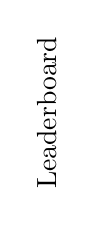
\begin{tikzpicture}\node[rotate=90] at (0,0){Leaderboard};\end{tikzpicture}}
&GIN                 & 0.526  0.051 & 96.485  0.252 & 55.255  1.527 & (+Lap)\!\!\! & 99.333  ~1.333 \\
&GraphSage           & 0.398  0.002 & 97.312  0.097 & 65.767  0.308 & (+Lap)\!\!\! & 99.933  ~0.467\\
&GAT                 & 0.384  0.007 & 95.535  0.205 & 64.223  0.455 & (+Lap)\!\!\! & 99.933  ~0.467 \\
&GCN                 & 0.367  0.011 & 90.705  0.218 & 55.710  0.381 & (+Lap)\!\!\!\!\! & \!\!\textbf{100.000}  ~\textbf{0.000}~ \\
&3WLGNN              & 0.303  0.068 & 95.075  0.961 & 59.175  1.593 &        & 95.700  \!\!\! 14.850 \\
&GatedGCN            & 0.214  0.006 & 97.340  0.143 & 67.312  0.311 & (+Lap)\!\!\! & 99.600  ~1.083 \\
&MPNN                & 0.145  0.007 & 97.690  0.220 & 70.860  0.270 &        & ~- \\
&PNA                 & 0.142  0.010 & \textbf{97.940}  \textbf{0.120} & 70.350  0.630 & &  ~- \\
\midrule
\multirow{3}{*}{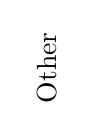
\begin{tikzpicture}\node[rotate=90] at (0,0){Other\!};\end{tikzpicture}}
&HIMP                & \!\!\!0.151  0.006 & ~~- & ~~- & & ~- \\
&DGN                 & \!\!\!0.168  0.003 & ~~- & \textbf{72.840}  \textbf{0.420} & & ~- \\
&GSN                 & \!\!\!0.108  0.018 & ~~- & ~~- & & ~- \\
\midrule
\multirow{2}{*}{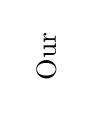
\begin{tikzpicture}\node[rotate=90] at (0,0){Our\!};\end{tikzpicture}}
&\crawl{}    & \textbf{0.101}  \textbf{0.003} & ~\textbf{97.978}  \textbf{ 0.079} & 68.106  0.340 & & \!\!\!\textbf{100.000}  ~\textbf{0.000} \\
&\crawl{}+VN & \textbf{0.088}  ~\textbf{0.003} & ~~- & ~~- & & ~- \\
\bottomrule
\end{tabular}
}
}
\end{tiny}
\end{center}
\vskip -0.1in
\end{table*}


\subsection{Experimental Setting}
We adopt the training procedure specified by \citet{dwivedi2020benchmarkgnns}.
In particular, the learning rate is initialized as  and decays with a factor of  if the performance on the validation set stagnates for  epochs.
The training stops once the learning rate falls below .
\citet{dwivedi2020benchmarkgnns} also specify that networks need to stay within parameter budgets of either 100K or 500K parameters.
This ensures a fairer comparison between different methods.
For \textsc{ZINC}, we use the larger budget of 500K parameters.
For the other three datasets we build \crawl{} models with the smaller budget of 100K.
The OGB Project does not specify a standardized training procedure or parameter budgets.
We use the same training procedure as for the previous datasets.
For MOLPCBA, we reduce the patience of the learning rate decay to 5  to decrease training time, which we generally limit to 12 hours.
We use the standard evaluators provided by OGB to measure the performance of the trained networks.

During training, we set the walk length to , except for MOLPCBA, where we use  to reduce the memory footprint.
For evaluation, we select the walk length  that yields the highest performance on the validation data.
This value is then used during testing.
All hyperparameters and the exact number of trainable parameters are listed in the appendix.
There, we also specify the sets of hyperparameters we searched for each dataset.


For each dataset, we train 5 models with different random seeds.
In all tables, we report the mean performance and standard deviation across those 5 models.
The output of each model depends on the sampled random walks.
Thus, we evaluate each model on 10 different seeds used for the generation of random walks and take the average of those runs as the model's performance.
Only on MOLPCBA we restrict the evaluation to 5 seeds for efficiency.
In the appendix we provide extended results that additionally specify the internal model deviation, that is, the impact of the random walks on the performance.
Since this internal model deviation is substantially lower than the differences between the models, they are comparatively insignificant when comparing \crawl{} to other models.




In several experiments we extend the network with a \emph{virtual node} (VN).
Intuitively, the VN is a special node that is connected to every node in the graph and uses its own update and message generation functions.
Adding such a virtual node is a common method to strengthen message passing GNNs on chemical prediction tasks.
We implemented the VN as an intermediate layer that updates the latent embeddings of all nodes between any two \crawl{} layers.
A formal definition is given in the appendix.
Note that it is not necessary to actually insert the VN into the graph and thus, it does not occur in the sampled random walks.


\subsection{Baselines}
We compare the results obtained with \crawl{} to a wide range of graph learning methods.
We report values that are currently listed on the leaderboard for the benchmark datasets as well as additional results from the literature that are not officially listed yet.
Our main baselines are numerous message passing GNN architectures that have been proposed in recent years (see Section \ref{relwork}), as well as a few others, such as an MPNN implemented by \citet{corso2020principal}.
Where available, we report the results for models trained with FLAG \cite{kong2020flag} which was proposed to improve the training of GNNs with adversarial data augmentation.
We also report results for non-neural graph embeddings combined with random forests that serve as a general baseline for GNNs.
In particular, we consider WEGL \cite{kolouri2020wasserstein} and Morgan Fingerprints \cite{doi:10.1021/ci100050t}.

For the CSL dataset we provide the accuracies achieved with positional encodings used as additional node features for the standard MPGNN baselines.
These features are based on Laplacian eigenvectors, as suggested by \citet{dwivedi2020benchmarkgnns}, and provide structural information about the graph. Without these extra features, MPGNNs cannot distinguish the 4-regular CSL graphs and achieve at most 10\% accuracy.
We do not use these additional features for \crawl{} networks. 

\subsection{Results}

Table \ref{zinc_results} provides our results on ZINC, MNIST, CIFAR10, and CSL.
On the ZINC dataset, \crawl{} achieves an MAE of 0.101.
This is approximately a 30\% improvement over the current first place (PNA) of the leaderboard.
When extending \crawl{} with virtual node layers, the result improves even further to 0.088 MAE.
On the MNIST dataset, \crawl{} also achieves the highest accuracy but with only a small margin to PNA which is the next best approach.
On CIFAR10, \crawl{} achieves the fourth highest accuracy among the eleven compared approaches.
On CSL, \crawl{} achieves an accuracy of 100\% which indicates that the task is comparatively easy for it.
None of the 5 trained \crawl{} models misclassified a single graph in the test folds.
Standard MPGNNs can only achieve more then 10\% accuracy when the additional positional encodings (+LAP) are provided.
Even with these features, only GCN achieves 100\% accuracy.
3WLGNN is theoretically capable of solving the task without additional node features.
However, it does not achieve 100\%, unlike \crawl{}.

Table \ref{ogb_results} provides the performance achieved on the OGB datasets MOLHIV and MOLPCBA.
Again, the provided baseline results are taken from the leaderboard of the OGB project.
On MOLHIV, we observed significant issues with overfitting.
\crawl{} outperforms popular GNN architectures such as GIN and GCN, but only ranks 11-th on the current leaderboard.
We point out that the current state-of-the-art for MOLHIV is Morgan Fingerprints, a handcrafted molecular fingerprint combined with a decision tree classifier.
Therefore, deep learning methods seem to generally struggle on this comparatively small dataset.

On MOLPCBA, \crawl{} yields state-of-the-art results.
Without using a virtual node, our method places second on the leaderboard and is only outperformed by GINE+(+VN).
When combining \crawl{} with a virtual node, the performance increases further and our approach places first.

Overall, \crawl{} performs very well on a variety of datasets across several domains.


\begin{table}[t]
\caption{Results achieved on MOLHIV and MOLPCBA. 
``+VN" indicates the usage of a virtual node. 
``+F" indicates the usage of FLAG \cite{kong2020flag}.}
\label{ogb_results}
\begin{center}
\begin{small}
\textsc{
\begin{tabular}{l|c|c}
\toprule
Method & MOLHIV & MOLPCBA \\
 & Test ROC-AUC & Test AP \\
\midrule
MFP         & \textbf{0.8060}  \textbf{0.0010} & 0.2054  0.0004 \\
WEGL        & 0.7757  0.0111 & - \\
GCN         & 0.7606  0.0097 & 0.2020  0.0024 \\
GCN+VN      & 0.7599  0.0119 & 0.2424  0.0034 \\
GCN+VN+F    & - & 0.2483  0.0037 \\
GIN         & 0.7558  0.0140 & 0.2266  0.0028 \\
GIN+VN      & 0.7707  0.0149 & 0.2703  0.0023 \\
GIN+VN+F    & 0.7748  0.0096 & 0.2834  0.0038 \\
DGCN        & 0.7858  0.0117 & 0.2745  0.0025 \\
DGCN+VN     & - & 0.2781  0.0038 \\
DGCN+F      & 0.7942  0.0120 & - \\
DGCN+VN+F   & - & 0.2842  0.0043 \\
GSN         & 0.7799  0.0100 & - \\
HIMP        & 0.7880  0.0082 & - \\
DGN         & 0.7970  0.0097 & - \\
PNA         & 0.7905  0.0132 & - \\
GINE+(+VN)  & 0.7880  0.0080 & 0.2917  0.0015 \\
\midrule
\crawl{}  & 0.7696  0.0167 & 0.2866  0.0016\\
\crawl{}\,+\,VN  & 0.7737  0.0099 & \textbf{0.2923}  \textbf{0.0024}\\
\bottomrule
\end{tabular} 
}
\end{small}
\end{center}
\vskip -0.1in
\end{table} 
\subsection{Ablation Study}
\label{sec:ablation study}

In an ablation study on the ZINC and CSL datasets, we evaluated the importance of the identity and adjacency encodings in the walk features and the effects of the two walk strategies.
We observed that each individual encoding significantly improves the results and the combination of both yields the best performance.
When looking at the walk strategies, non-backtracking walks perform as good or better than uniform walks for all tested node feature variants in the ablation study.
On ZINC with the full walk features, both strategies yield virtually identical results.
The detailed results are provided in Appendix C.

     \section{Expressiveness}
\label{sec:expressiveness}

In this section, we report on theoretical results
comparing the expressiveness of \crawl{} with that of other
methods. The additional strength of \crawl{} is mainly derived from the fact
that it detects small subgraphs (of size determined by the window size
hyperparameter ) and can sample such subgraphs from a non-uniform, but
well-defined, distribution determined by the random walks. In this
sense, it is similar to network analysis techniques based on motif
detection \cite{alo07} and graph kernels based on counting subgraphs, such as the graphlet kernel \cite{shevispet+09}.

The following results are concerned with the basic question which graphs
can be distinguished by the various methods, assuming that optimal
parameters for the models are available. They do not discuss how such
parameters can be learned. This limits the scope of these results,
but they still give useful intuition about the different approaches.



It is known that the expressiveness of GNNs corresponds exactly to
that of the 1-dimensional Weisfeiler-Leman algorithm (1-WL)
\cite{MorrisAAAI19,Keyulu18}, in the sense that two graphs are
distinguished by 1-WL if and only if they can be distinguished by a
GNN. 
It is also known that higher-dimensional versions of WL characterize the expressiveness of higher-order GNNs \cite{MorrisAAAI19}.


\newtheorem{theorem}{Theorem}

\begin{theorem}\label{theo:1}
 \hphantom\\
  \begin{enumerate}
  \item For every  there are graphs that are distinguishable
    by \crawl{}, but not
    by -WL (and hence not by -dimensional GNNs).
  \item There are graphs that are distinguishable by 1-WL (and hence
    by GNNs), but not by \crawl{}.
  \end{enumerate}
\end{theorem}

We state a precise quantitative version of the theorem and give a
proof in Appendix~D. Let us just note that for
{assertion (1)} we need a window size  and walk length 
quadratic in , and for (2) we can allow \crawl\ to use a window
size and path length linear in the size of the graphs.
It can also be shown that
\crawl{} with a window size polynomial in the size of the graphlets is strictly more expressive than graphlet kernels. We omit the precise result, which can be proved similarly to Theorem~\ref{theo:1}(1), due to space
limitations.


Let us finally remark that the expressiveness of GNNs can be
considerably strengthened by adding a random node initialization
\cite{abbceygroluk20,SatoRandom2020}. The same can be done for \crawl{},
but so far the need for such a strengthening (at the cost of a higher
variance) did not arise.



     \section{Conclusion}
\label{conclusion}

We have introduced a novel neural network architecture \crawl{} for graph learning that is based on random walks and 1D CNNs.
Thus, \crawl{} is fundamentally different from standard graph neural networks.
We demonstrated that this approach works very well across a variety of graph level tasks and is able to outperform state-of-the-art GNNs.
By construction, \crawl{} can detect arbitrary substructures up to the size of its local window.
In particular, on the regular graphs of CSL where pure MPGNNs fail because of the lack of expressiveness, \crawl{} is able to extract useful features and solve this task.


Future work includes extending the experimental framework to node-level tasks and to motif counting. 
In both cases, one needs to scale \crawl{} to work on individual large graphs instead of many medium sized ones.
On those large graphs the current implementation struggles to stay within the available RAM of most GPUs.
We expect the quality of \crawl{}'s predictions in those settings to be at least comparable to that of message passing based approaches.




\crawl{} can be viewed as an attempt
to process random walks and the structures they induce with end-to-end neural networks.
The strong empirical performance demonstrates the potential of this general approach.
However, many variations remain to be explored, including different walk strategies, variations in the walk features, and alternative pooling functions for pooling walklet embeddings into nodes or edges. In view of the incomparability of the expressiveness of GNNs and \crawl{}, hybrid approaches that interleave \crawl{} layers and GNN layers seem attractive as well.
Beyond plain 1D-CNNs, other deep learning architectures for sequential data, such as transformer networks, could be used to process random walks.




\section*{Acknowledgements}
This work is supported by the German Research Foundation (DFG) under grant GR 1492/16-1.     
    \bibliographystyle{abbrvnat}
    \bibliography{bibliography}
    
    \pagebreak
    \appendix
    \section{Extended Results}
\subsection{Additional Experiments}
\label{social_exp}

In this section we evaluate \crawl{} on commonly used benchmark datasets from the domain of social networks.
We use a subset from the \mbox{TUDataset} \citep{Morris+2020}, a list of typically small graph datasets from different domains e.g. chemistry, bioinformatics, and social networks.
We focus on three datasets originally proposed by \citet{yanardag2015deep}: COLLAB, a scientific collaboration dataset, IMDB-MULTI, a multiclass dataset of movie collaboration of actors/actresses, and REDDIT-BIN, a balanced binary classification dataset of Reddit users which discussed together in a thread.
These datasets do not have any node or edge features and the tasks have to be solved purely with the structure of the graphs. 



We stick to the experimental protocol suggested by \citet{Keyulu18}.
Specifically, we perform a 10-fold cross validation.
Each dataset is split into 10 stratified folds.
We perform 10 training runs where each split is used as test data once, while the remaining 9 are used for training.
We then select the epoch with the highest mean test accuracy across all 10 runs.
We report this mean test accuracy as the final result.
This is not the most realistic setup for simulating real world tasks, since there is no clean split between validation and test data.
But in fact, it is the most commonly used experimental setup for these datasets and is mainly justified by the comparatively small number of graphs.
Therefore, we adopt the same procedure for the sake of comparability to the previous literature.
For COLLAB and IMDB-MULTI we use the same 10-fold split used by \citet{zhang2018end}.
For REDDIT-BIN we computed our own stratified splits.
We also computed separate stratified 10-fold splits for hyperparameter tuning.

We adapt the training procedure of \crawl{} towards this setup.
Here, the learning rate decays with a factor of 0.5 in fixed intervals.
These intervals are chosen to be 20 epochs on COLLAB and REDDIT-BINARY and as 50 epochs on IMDB-MULTI.
We train for 200 epochs on COLLAB and REDDIT-BINARY and for 500 epochs on IMDB-MULTI.
This ensures a consistent learning rate profile across all 10 runs for each dataset.

Table \ref{social_results} reports the achieved accuracy of \crawl{} and several key baselines.
For the baselines, we provide the results as reported in the literature.
For comparability, we only report values for baselines with the same experimental protocol.
On IMDB-MULTI, the smallest of the three datasets, \crawl{} yields a slightly lower accuracy then most baselines.
On COLLAB, our method performs similarly to standard MPGNN architectures, such as GIN.
\crawl{} outperforms all baselines that report values for REDDIT-BIN.
Note that GSN, the method with the best results on COLLAB and IMDB-MULTI, does not scale as well as \crawl{} and is infeasible for REDDIT-BIN.


\begin{table*}[t]
\caption{Accuracy on Social Datasets.}
\label{social_results}
\begin{center}
\begin{small}
\begin{tabular}{l r|c|c|c}
\toprule
Method      && COLLAB & IMDB-MULTI & REDDIT-BIN \\
            && Test Acc & Test Acc & Test Acc \\
\midrule
WL-Kernel   &\citep{shervashidze2011weisfeiler}& 78.9  1.9 & 50.9  3.8 & 81.0  3.1 \\
WEGL        &\citep{kolouri2020wasserstein}& 79.8  1.5 & 52.0  4.1 & 92.0  0.8 \\
GNTK        &\citep{NEURIPS2019_663fd3c5}& 83.6  1.0 & 52.8  4.6 & - \\
DGCNN       &\citep{zhang2018end}& 73.8  0.5 & 47.8  0.9 & - \\
3WLGNN      &\citep{maron2019provably}& 80.7  1.7 & 50.5  3.6 & - \\
GIN         &\citep{Keyulu18}& 80.2  1.9 & 52.3  2.8 & 92.4  2.5 \\
GSN         &\citep{bouritsas2020improving}& \textbf{85.5}  \textbf{1.2} & \textbf{54.3}  \textbf{3.3} & - \\

\midrule
\crawl{}    &&   &  & \textbf{93.15\%}  \textbf{1.21} \\
\bottomrule
\end{tabular}
\end{small}
\end{center}
\vskip -0.1in
\end{table*} \subsection{Detailed Results for all Experiments}

Table \ref{extended_results} provides the full results from our experimental evaluation.
It reports the performance on the train, validation and test data.


Recall that the output of \crawl{} is a random variable.
The predictions for a given input graph may vary when different random walks are sampled.
To quantify this additional source of randomness, we measure two deviations for each experiment: 
The cross model deviation (CMD) and the internal model deviation (IMD).
For clarity, let us define these terms formally.
For each experiment, we perform  training runs with different random seeds.
Let  be the model obtained in the -th training run with .
When evaluating (both on test and validation data), we evaluate each model  times, with different random walks in each evaluation run.
Let  measure the performance achieved by the model  in its -th evaluation run.
Note that the unit of  varies between experiments (Accuracy, MAE, ).
We formally define the \emph{internal model deviation} as

where  is the standard deviation of a given distribution.
Intuitively, the IMD measures how much the performance of a trained model varies when applying it multiple times to the same input.
It quantifies how the model performance depends on the random walks that are sampled during evaluation.

We formally define the \emph{cross model deviation} as

The CMD measures the deviation of the average model performance between different training runs.
It therefore quantifies how the model performance depends on the random initialization of the network parameters before training.

In the main section, we only reported the CMD for simplicity.
Note that the CMD is significantly larger then the IMD across all experiments.
Therefore, trained \crawl{} models can reliably produce high quality predictions, despite their dependence on randomly sampled walks.

\begin{table*}[t]
\caption{Extended results for \crawl{} on all datasets. Note that different metrics are used to measure the performance on the datasets. ``+VN" indicates models with an additional virtual node. For each experiment we provide the cross model deviation (CMD) and the internal model deviation (IMD).}
\label{extended_results}
\begin{center}
\begin{tiny}
\textsc{
\begin{tabular}{l|l|r|r|r|r|r|r|r|r}
\toprule
Dataset / Model & Metric & \multicolumn{3}{c|}{Test} & \multicolumn{3}{c|}{Validation} & \multicolumn{2}{c}{Train} \\
        & & Score & CMD & IMD & Score & CMD & IMD & Score & CMD \\
\midrule 
ZINC        & MAE & 0.10083 & 0.00299 & 0.00157 & 0.12619 & 0.00166 & 0.00113 & 0.04818 & 0.00439 \\
ZINC+VN     & MAE & 0.08762 & 0.00326 & 0.00125 & 0.11362 & 0.00433 & 0.00107 & 0.05743 & 0.00539 \\
CIFAR10     & Acc. & 0.68106 & 0.00340 & 0.00147 & 0.68961 & 0.00523 & 0.00230 & 0.79197 & 0.00913 \\
MNIST       & Acc.& 0.97978 & 0.00079 & 0.00070 & 0.98054 & 0.00086 & 0.00068 & 0.98680 & 0.00198 \\
CSL         & Acc.& 1.00000 & 0.00000 & 0.00000 & 1.00000 & 0.00000 & 0.00000 & 1.00000 & 0.00000 \\
\midrule
MOLHIV      & ROC-AUC & 0.76956 & 0.01669 & 0.00175 & 0.81737 & 0.01592 & 0.00196 & 0.86264 & 0.04626 \\
MOLHIV+VN   & ROC-AUC & 0.77376 & 0.00990 & 0.00195 & 0.82189 & 0.00434 & 0.00134 & 0.86840 & 0.03913 \\
MOLPCBA     & AP & 0.28662 & 0.00163 & 0.00062 & 0.29310 & 0.00157 & 0.00056 & 0.50987 & 0.01113 \\
MOLPCBA+VN  & AP & 0.29230 & 0.00235 & 0.00043 & 0.29647 & 0.00413 & 0.00056 & 0.51144 & 0.00999 \\
\midrule
COLLAB      & Acc. & 0.80580 & 0.01481 & 0.00670 & - & - & - & 0.82289 & 0.00267 \\
IMDB-MULTI  & Acc. & 0.48907 & 0.02715 & 0.01290 & - & - & - & 0.50030 & 0.00730 \\
REDDIT-BIN  & Acc. & 0.93150 & 0.01210 & 0.00300 & - & - & - & 0.93894 & 0.00590 \\
\bottomrule
\end{tabular}
}
\end{tiny}
\end{center}
\vskip -0.1in
\end{table*}      \section{Model and Setup Details}
\subsection{Hyperparameters}
Table \ref{hyper_param} provides the hyperparameters used in each experiment.
These consist of the following:
\begin{itemize}
    \item The number of layers . 
    We tried out  on all datasets, except for MOLPCBA, where we searched through .
    \item The latent state size . On ZINC, CIFAR10, MNIST and CSL we chose sizes that would roughly use the chosen parameter budgets. On MOLHIV, COLLAB, IMDB-MULTI and REDDIT-BIN we searched through  and for MOLPCBA we chose the largest feasible size for our hardware . 
    \item The global pooling function (either \emph{mean} or \emph{sum})
    \item The architecture of the final output network (either \emph{mlp} or \emph{linear})
    \item The number of random walk steps during training () and evaluation (). 
    By default we set . 
    Only on MOLPCBA we set  to stay within GPU memory limits.
    We searched through  on the validation data of all datasets.
    \item The probability of starting a walk from each node during training .
    We choose  by default.
    On MOLPCBA we set  to stay within GPU memory limits.
    On MOLHIV we searched through  to reduce overfitting.
    \item The walk strategy (either \emph{uniform} (un) or \emph{non-backtracking} (nb))
    \item The number of evaluation runs with different random walks for validation () and testing ().
    \item The dropout rate. We searched through \{0.0, 0.5\}. A dropout layer is placed behind the hidden layer of the update MLP  in each \crawl{} layer.
    \item The initial learning rate  was chosen as  in all experiments.
    \item The patience for learning rate decay (with a factor of ) is  by default. It is set to  on MOLPCBA to decrease runtime.
    For CSL it is set to  due to the small dataset size.
    \item For the batch size we searched through  for most datasets.
    We chose a batch size of 120 for CSL, which combines all of the training data into one batch.
\end{itemize}
\begin{table*}[t]
\caption{Configurations used for each dataset.}
\label{hyper_param}
\begin{center}
\begin{tiny}
\begin{tabular}{l|c|c|c|c|c|c|c|c|c}
\toprule
 & ZINC & CIFAR10 & MNIST & CSL & MOLHIV & MOLPCBA & COLLAB & IMDB-M & REDDIT-B \\
\midrule
 & 3 & 3 & 3 & 2 & 3 & 5 & 3 & 3 & 3 \\
 & 100 & 50 & 50 & 64 & 64 & 250 & 64 & 64 & 64 \\
pool & sum & mean & mean & mean & mean & mean & mean & mean & mean \\
out & mlp & mlp & mlp & mlp & linear & linear & mlp & mlp & mlp \\
  & 50 & 50 & 50 & 50 & 50 & 40 & 50 & 50 & 50 \\
  & 100 & 100 & 100 & 100 & 100 & 100 & 50 & 50 & 50 \\
 & 1 & 1 & 1 & 1 & 0.1 & 0.25 & 1 & 1 & 1 \\
walk strat.\! & nb & nb & nb & nb & nb & nb & nb & nb & nb \\
 & 2 & 2 & 2 & 5 & 5 & 1 & - & - & - \\
 & 10 & 10 & 10 & 10 & 10 & 5 & 5 & 5 & 5 \\
dropout & 0.0 & 0.5 & 0.5 & 0.5 & 0.5 & 0.5 & 0.5 & 0.5 & 0.5 \\
 & 0.001 & 0.001 & 0.001 & 0.001 & 0.001 & 0.001 & 0.001 & 0.001 & 0.001 \\
patience & 10 & 10 & 10 & 20 & 10 & 5 & - & - & - \\
batch size & 50 & 50 & 50 & 50 & 50 & 75 & 50 & 50 & 50 \\
\bottomrule
\end{tabular}
\end{tiny}
\end{center}
\vskip -0.1in
\end{table*}


\subsection{Model Size and Runtime}
Table \ref{param_count} provides the number of trainable parameters in each model.
Additionally, we report the runtime observed during training.
All experiments were run on a machine with 32GB RAM, an Intel Xeon 8160 CPU and an Nvidia Tesla V100 GPU with 16GB GPU memory.

Note that we enforced a time limit of 12 hours when training on MOLPCBA.
However, several models finished training in under 12 hours, hence, the mean runtime on MOLPCBA is less than this limit.
\begin{table}[t]
\caption{Number of parameters and runtime for each model in our experiments. 
The reported times are averaged over all training runs and include the time used to perform a validation run after each training epoch.}
\label{param_count}
\vskip 0.15in
\begin{center}
\textsc{
\begin{tabular}{l|r|r|r}
\toprule
Model & \#Param. &
\!\!\!\!\begin{tabular}{c}Time/Epoch\\\tiny{(MM:SS.00)}\end{tabular}\!\!\! &
\!\!\!\!\begin{tabular}{c}Train Time\\\tiny{(HH:MM:SS)}\end{tabular}\!\!\! \\
\midrule
ZINC & 423,901 & 00:20.66 & 01:21:44 \\
ZINC + VN & 464,301 & 00:26.01 & 01:36:46 \\
CIFAR10 & 109,760 & 01:58.69 & 04:56:26 \\
MNIST & 109,160 & 01:46.17 & 04:45:37 \\
CSL & 110,794 & 00:00.26 & 00:00:57 \\
MOLHIV & 206,465 & 00:29.44 & 00:48:17 \\
MOLHIV + VN & 223,105 & 00:32.16 & 00:52:57 \\
MOLPCBA & 4,372,128 & 06:42.28 & 11:41:21 \\
MOLPCBA + VN & 4,874,128 & 07:13.71 & 11:07:15 \\
COLLAB & 173,315 & 00:14.35 & 00:47:50 \\
IMDB-MULTI & 173,315 & 00:01.63 & 00:13:35 \\
REDDIT-BIN & 173,185 & 00:36.48 & 02:01:35 \\
\bottomrule
\end{tabular}
}
\end{center}
\vskip -0.1in
\end{table} 

\subsection{Virtual Node}
\label{vn}
\citet{GilmerSRVD17}, \citet{li2017learning}, and \citet{ishiguro2019graph} suggested the use of a \emph{virtual node} to enhance GNNs for chemical datasets.
Intuitively, a special node is inserted into the graph that is connected to all other nodes.
This node aggregates the states of all other nodes and uses this information to update its own state.
The virtual node has its own distinct update function, that is not shared by other nodes.
The updated state is then sent back to all nodes in the graph.
Effectively, a virtual node allows global information flow after each layer.


Formally, a virtual node updates a latent state , where  is computed after the -th layer and  is initialized as a zero vector.
The update procedure is defined by:

Here,  is a trainable MLP and  is the latent node embedding computed by the -th \crawl{} layer.
 is an updated node embedding that is used as the input for the next \crawl{} layer instead of .
In our experiments, we choose  to contain a single hidden layer of dimension .
When using a virtual node, we perform this update step after every \crawl{} layer, except for the last one.

Note that we view the virtual node as an intermediate update step that is placed between our \crawl{} layers to allow for global communication between nodes.
No additional node is actually added to the graph and, most importantly, the ``virtual node" does not occur in the random walks sampled by \crawl{}.

\subsection{Cross Validation on CSL}
Let us briefly discuss the experimental protocol used for the CSL dataset.
Unlike the other benchmark datasets provided by \citet{dwivedi2020benchmarkgnns}, CSL is evaluated with 5-fold cross-validation.
We use the 5-fold split \citet{dwivedi2020benchmarkgnns} provide in their repository.
In each training run, three folds are used for training and one is used for validation.
After training, the remaining fold is used for testing.

Finally, Figure \ref{fig:skiplink} provides an example of two skip-link graphs.
The task of CSL is to classify such graphs by their isomorphism class.
\begin{figure}
    \centering
\includegraphics[width=0.7\textwidth]{picture_skiplink.pdf}
    \caption{Two cyclic skip-link graphs \citep[see][]{murphy2019relational} \textbf{}with 11 nodes and a skip distance of 2 and 3 respectively.}
    \label{fig:skiplink}
\end{figure}     \section{Ablation Study}
\label{ablation study}
\begin{table*}[t]
\caption{Results of our ablation study. Node features , edge features , adjacency encoding , and identity encoding . Walk strategies no-backtrack (NB) and uniform (UN).}
\label{ablation_results}
\begin{center}
\begin{small}
\textsc{
\begin{tabular}{l|c|r|r}
\toprule
Features & Walk Strat. & ZINC (MAE) & CSL (Acc) \\
\midrule
 +                & NB & 0.17655  0.00303 & 0.12000  0.08055 \\
 +                & UN & 0.25827  0.02115 & 0.12000  0.08055 \\ \midrule
 +  +          & NB & 0.10636  0.00326 & 1.00000  0.00000 \\
 +  +          & UN & 0.11053  0.00417 & 0.98000  0.02357 \\ \midrule
 +  +          & NB & 0.11094  0.00398 & 0.96267  0.02175 \\
 +  +          & UN & 0.13297  0.00769 & 0.75200  0.03284 \\ \midrule
 +  +  +    & NB & 0.10083  0.00299 & 1.00000  0.00000 \\
 +  +  +    & UN & 0.09932  0.00402 & 0.96533  0.02050 \\
\bottomrule
\end{tabular} 
}
\end{small}
\end{center}
\vskip -0.1in
\end{table*} We perform an ablation study to understand how the key aspects of \crawl{} influence the empirical performance.
We aim to answer two main questions:
\begin{itemize}
    \item How useful are the identity and adjacency features we construct for the walks?
    \item How do different strategies for sampling random walks impact the performance?
\end{itemize}

Here, we use the ZINC and CSL datasets to answer these questions empirically.
We trained multiple versions of \crawl{} with varying amounts of structural features used in the walk feature matrices.
The simplest version only uses the sequences of node and edge features without any structural information.
We then trained versions that add either the adjacency encoding or the identity encoding.
Finally, we measure the performance of the standard \crawl{} architecture, where both encodings are incorporated into the walk feature matrices.
For each version, we measure the performance with both walk strategies.

On both datasets, the experimental setup and hyperparameters are identical to those used in the previous experiments on both datasets.
In particular, we train five models with different seeds and provide the average performance as well as the standard deviation across models.
Note that we repeat the experiment independently for each walk strategy.
Switching strategies between training and evaluation does not yield good results.

Table \ref{ablation_results} reports the performance of each studied version of \crawl{}.
On ZINC, the networks without any structural encoding yield the worst predictions.
Adding either the adjacency or the identity encoding improves the results substantially.
The best results are obtained when both encodings are utilized.
Curiously, the uniform walks actually yield marginally better results on the test split when all structural features are considered.
On the validation split, the non-backtracking strategy performs slightly better, which is why it was used in our main experiments.

On CSL, the adjacency feature is sufficient to reach 100\%, but adding the identity feature does not decrease this performance.
The non-backtracking walks perform consistently better than the uniform walks, which did not achieve 100\% on this dataset.
Finally, we point out that the network with no structural features should not be able to achieve more than 10\% on CSL if the labels in the folds were balanced.
However, we noticed that the splits provided by \citet{dwivedi2020benchmarkgnns} are not stratified and a network can achieve a mean accuracy of roughly 12\% through random guessing.     \section{Theory}
\label{appendix:proof}

We need some additional notation. Throughout the paper, graphs are 
undirected and simple (that is, without self-loops and parallel edges).\footnote{It is possible to simulate directed edges and parallel edges through edge labels and loops through node labels, but so far, we have only worked with undirected simple, though possibly labeled graphs.}
In this appendix, all graphs will be unlabeled, and we assume that they have no isolated nodes, which enables us to
start a random walk from every node. We denote the edge set of a
graph  by  and the node set by . The \emph{order}
 of  is the number of nodes, that is,
.
For a set , the
\emph{induced subgraph}  is the graph with node set  and
edge set .
A walk of length  in  is a sequence
 such that  for . The walk is \emph{non-backtracking}
if for  we have
 unless the degree of vertex  is .








Before we prove the theorem, let us precisely specify what it means that \crawl{}
distinguishes two graphs. Recall that \crawl{} has three (walk related) hyperparameters:
\begin{itemize}
\item the \emph{window size} ;
\item the \emph{walk length} ;
\item the \emph{samples size} .
\end{itemize}
Recall furthermore that with every walk  we associate a
\emph{walk feature matrix} . For
, the first  entries of the -th row of 
describe the label of the node , the next  entries the
label of the edge  ( for ), the following 
entries are indicators for the equalities between  and the
nodes  for  ( if ,  if
 or ), and the remaining  entries are
indicators for the adjacencies between  and the nodes
 for  ( if  are adjacent in ,
 if  or  are non-adjacent; note that
 are always be adjacent because  is a walk in ). In
this section, we always consider unlabeled graphs and therefore
obtain walk feature matrices . We
denote the entries of the matrix  by  and the rows by
. So .
We denote the walk feature matrix of a walk  by . It is
immediate from the definitions that for walks
 in graphs  with
feature matrices , we have:
\begin{enumerate}
  \item
  if  for  then the mapping  for
 is an isomorphism from the induced subgraph
 to the induced subgraph
;
\item 
if the mapping  for
 is an isomorphism from the induced subgraph
 to the induced subgraph
, then  for .
\end{enumerate}
The reason that we need to include the vertices
 and  into the subgraphs in (2) is that row  of the feature matrix records edges
and equalities between  and .

For every graph  we denote the distribution of random walks on 
starting from a node chosen uniformly at random by  and
 for the
non-backtracking walks. We let
 and ) be the push-forward distributions on
, that is, for every
 we let

A \crawl{} run on  takes  samples from . So to
distinguish two graphs , \crawl{} must detect that the
distributions  are distinct using  samples.

As a warm-up, let us prove the following simple result.
\setcounter{theorem}{1}
\begin{theorem}\label{theo:a1}
  Let  be a cycle of length  and  the disjoint union of two
  cycles of length . Then  and
   cannot be distinguished by \crawl{} with window size 
  (for any choice of parameters  and ).
\end{theorem}

\begin{proof}
  With a window size smaller than the length of the shortest
  cycle, the graph \crawl{} sees in its window is always a path. Thus for every walk  in either  or 
  the feature matrix  only depends on the backtracking pattern
  of . This means that  .
\end{proof}

It is worth noting that the graphs  of Theorem~\ref{theo:a1} can
be distinguished by -WL (the 2-dimensional Weisfeiler-Leman
algorithm), but not by -WL.

Proving that two graphs  have identical feature-matrix distributions
 is the ultimate way of proving that they are not
distinguishable by \crawl{}. Yet for more interesting graphs, we rarely
have identical feature-matrix distributions. However, if the
distributions are sufficiently close we will still not be able to
distinguish them. To quantify closeness, we use the \emph{total variation
distance} of the distributions. Recall that the total variation distance between two
probability distributions  on the same finite sample space
 is

It is known that the total variation distance is half the
-distance between the distributions, that is,

Let . We say that two graphs  are
\emph{-indistinguishable} by \crawl{} with window size ,
walk length , and sample size  if

The rationale behind this definition is that if
 then for every
property of feature matrices that \crawl{} may want to use to
distinguish the graphs, the expected numbers of samples with this
property that \crawl{} sees in both graphs are close together
(assuming  is small).

Often, we want to make asymptotic statements, where we have two
families of graphs  and , typically of
order , and classes  of functions, such
as the class  of logarithmic or the class  of
polynomial functions. We say that  and
 are \emph{indistinguishable} by \crawl{} with window
size , walk length , and sample size  if for all 
and all  there is an  such that 
are -indistinguishable by \crawl{} with window size ,
walk length , and sample size .

We could make similar definitions for distinguishability, but we omit
them here and deal with distinguishability in an ad-hoc fashion (in
the following subsection). 


\subsection{Proof of Theorem 1(1)}

Here is a precise quantitative version of the theorem.

\begin{theorem}\label{theo:1-1}
  For all  there are families of graphs ,
   of order  that are distinguishable by \crawl{} with
  window size , walk length , and samples size
  , but not by -WL (and hence not by -dimensional GNNs).
\end{theorem}


Fortunately, to prove this theorem we do not need to know any details
about the Weisfeiler-Leman algorithm (the interested reader is
deferred to \cite{kie20}). We can use the following
well-known inexpressibility result as a black box.

\begin{theorem}[\citet{caifurimm92}]\label{theo:cfi}
  For all  there are graphs  such that
  , the graphs  and  are -regular, and -WL cannot distinguish  and .
\end{theorem}


It is a well-known fact that the \emph{cover time} of a connected
graph of order  with  edges, that is, the expected time it takes
a random walk starting from a random node to visit all nodes of
the graph, is bounded from above by  \cite{alekarlip+79}. By Markov's
inequality, a path of length  visits all nodes with
probability at least . Sampling several such paths, we can bring
the success probability arbitrarily close to .

\begin{proof}[Proof of Theorem 1(1)]
  Let  and let  be
the graphs obtained from the Theorem~\ref{theo:cfi}. Let
. For every , we let  be the
disjoint union of  with a path of length , and let 
be defined in the same way from . Then .

  Let  be the number of edges of the -regular
graphs  and , and let . This
will be our window size, and in fact also our walk length: 
. Let . We choose a sufficiently large
 to make sure that a sample of  nodes from 
or  contains sufficiently many nodes in the subset
 resp.\ . Then, if we
sample  paths of length  from , with probability at
least , one of these paths covers . This means that  random walks of length 
will detect the subgraphs , and as the window size  is
equal to , these subgraphs will appear in the feature
matrix. Since the subgraph  does not appear as a subgraph of
, this means that with probability at least ,
\crawl{} can distinguish the two graphs.
\end{proof}

\begin{figure}
  \centering
  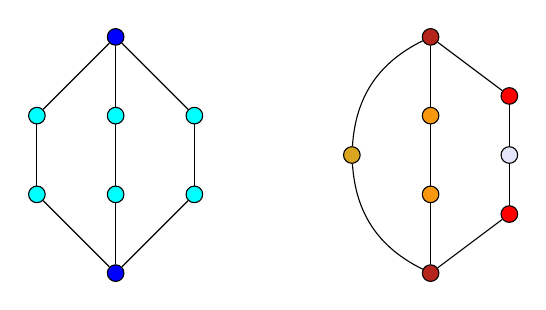
\begin{tikzpicture}[
  vertex/.style={circle,draw,inner sep = 0pt, minimum size=6pt},
  ]
  \begin{scope}
    \node[vertex,fill=Blue] (v1) at (0,0) {}; 
    \node[vertex,fill=Cyan] (v2) at (-1,1) {}; 
    \node[vertex,fill=Cyan] (v3) at (0,1) {}; 
    \node[vertex,fill=Cyan] (v4) at (1,1) {}; 
    \node[vertex,fill=Cyan] (v5) at (-1,2) {}; 
    \node[vertex,fill=Cyan] (v6) at (0,2) {}; 
    \node[vertex,fill=Cyan] (v7) at (1,2) {};
    \node[vertex,fill=Blue] (v8) at (0,3) {};

    \draw (v1) edge (v2) edge (v3) edge (v4) (v2) edge (v5) (v3) edge
    (v6) (v4) edge (v7) (v8) edge (v5) edge (v6) edge (v7);

    \node at (-1,3) {};
  \end{scope}

    \begin{scope}[xshift=4cm]
    \node[vertex,fill=BrickRed] (v1) at (0,0) {}; 
    \node[vertex,fill=Goldenrod] (v2) at (-1,1.5) {}; 
    \node[vertex,fill=YellowOrange] (v3) at (0,1) {}; 
    \node[vertex,fill=Red] (v4) at (1,0.75) {}; 
    \node[vertex,fill=YellowOrange] (v5) at (0,2) {}; 
    \node[vertex,fill=Lavender] (v6) at (1,1.5) {}; 
    \node[vertex,fill=Red] (v7) at (1,2.25) {};
    \node[vertex,fill=BrickRed] (v8) at (0,3) {};

    \draw (v1) edge[bend left] (v2) edge (v3) edge (v4) (v3) edge (v5) (v4) edge
    (v6) (v6) edge (v7) (v8) edge[bend right] (v2) edge (v5) edge (v7);

    \node at (-1,3) {};
  \end{scope}

  \end{tikzpicture}
  \caption{The graphs  and  in the proof of
    Theorem~\ref{theo:a2} with their stable coloring computed by -WL}
  \label{fig:3paths}
\end{figure}

\subsection{Proof of Theorem 1(2)}

To prove the second part of the theorem, it will be necessary to
briefly review the \emph{1-dimensional Weisfeiler-Leman algorithm
  (-WL)}, which is also known as \emph{color refinement} and as
\emph{naive node classification}. The algorithm iteratively computes
a partition of the nodes of its input graph. It is convenient to
think of the classes of the partition as colors of the
nodes. Initially, all nodes have the same color. Then in each
iteration step, for all colors  in the current coloring and all
nodes  of color , the nodes  and  get different colors
in the new coloring if there is some color  such that  and 
have different numbers of neighbors of color . This refinement
process is repeated until the coloring is \emph{stable}, that is, any
two nodes  of the same color  have the same number of
neighbors of any color . We say that -WL \emph{distinguishes}
two graphs  if, after running the algorithm on the disjoint
union  of the two graphs, in the stable coloring of
 there is a color  such that  and  have a different
number of nodes of color .


For the results so far, it has not mattered if we allowed backtracking
or not. Here, it makes a big difference. For the non-backtracking
version, we obtain a stronger result with an easier proof. The
following theorem is a precise quantitative statement of Theorem 1(2).

\begin{theorem}\label{theo:a2}
  There are families ,  of graphs of
  order  with the following properties.
  \begin{enumerate}
  \item For all , -WL distinguishes  and .
  \item ,  are indistinguishable by
    the non-backtracking version of \crawl{} with window size 
    (regardless of the walk length and sample size).
  \item   are indistinguishable by
    \crawl{} with walk length ,
    and samples size  (regardless of the window size).
    \end{enumerate}
\end{theorem}


\begin{proof}
  The graphs  and  both consist of three internally
  disjoint paths with the same endnodes  and . In  the lengths of
  all three paths is . In , the length of the
  paths is  (see
  Figure~\ref{fig:3paths}). 
  
  
  \medskip
  It is easy to see that -WL
distinguishes the two graphs. 

\medskip
To prove (2), 
let . Then the length of the shortest
cycle in ,  is . Now consider a non-backtracking walk
 in either  or  (of arbitrary length
). Then for all  and  with  we have
, and unless , there is no edge  between  and
. Thus  for all walks  of the same length ,
and since it does not matter which of the two graphs  the
walks are from. It follows that .

\medskip
Before we prove (3), we remark that the backtracking version of \crawl{} can distinguish
 and  with a constant window size
, walk length , and samples size . The reason
is that by going back and forth between a node and all its
neighbors within its window, \crawl{} can distinguish the two degree-
nodes  from the remaining degree- nodes. Thus, the feature matrix reflects traversal times between degree-3 nodes, and the distribution of traversal times is different in  and .
With sufficiently many samples, \crawl{} can detect this.

So, let us turn to the proof that with walks of linear length this is not possible, that is, assertion (3). 
The reason for this is simple:
random walks of length  are very unlikely to traverse a path
of length at least  from  to . It is well known that the expected
traversal time is  (this follows from the analysis of the
gambler's ruin problem). However, this does not suffice for us, we
need to bound the probability that a path of length  is a
traversal. Using a standard, Chernoff type tail bound, it is
straightforward to prove that for every constant
 there is a constant  such that the probability that a
random walk of length  in either  or  visits both 
and  is at most
. As only walks visiting both  and  can
differentiate between the two graphs, this gives us an upper bound of
 for the total variation distance between  and
. 
\end{proof}

 
\end{document}
